\subsection*{AND-gate}
\label{volumenkontrol-design-and}

De to AND-gates er designet med diskrete komponenter, fremfor en integreret kreds. AND-gaten fungerer ved at holde udgangen høj, når begge indgange er høje. På AND-gaten til venstre på figur \ref{fig:volumenkontrol_diagram}, er et højt udgangsniveau $\sim$0,6 V, dette skyldes at der på udgangen af gaten er en transistors basis-emitter diode til stel. Er blot den ene af indgangene lave, vil den trække udgangen til stel gennem den tilhørende diode, BAT85 \cite{bat85-datablad}. Databladet for BAT85 beskriver en sammenhæng mellem en diode spænding på 0,24 V og en strøm gennem den på 0,1 mA, dette resultere i en Pull-up modstand beregnet i ligning (\ref{equ:and-gate1}).

\begin{equation}
\label{equ:and-gate1}
V_{CC} - V_D = R_{15} \cdot I_F = 5~\mathrm{V} - 0,24~\mathrm{V} = R_{15} \cdot 0,1~\mathrm{mA} \Rightarrow R_{15} = 47,6~\mathrm{k}\ohm
\end{equation}

Udgangen af AND-gaten vil altså ikke kunne bliver højere end 0,24 V, ved lavt output.

\clearpage
\subsection*{Tæller og displaydriver}
\label{volumenkontrol-design-taeller}

\begin{figure}[h]
\centering
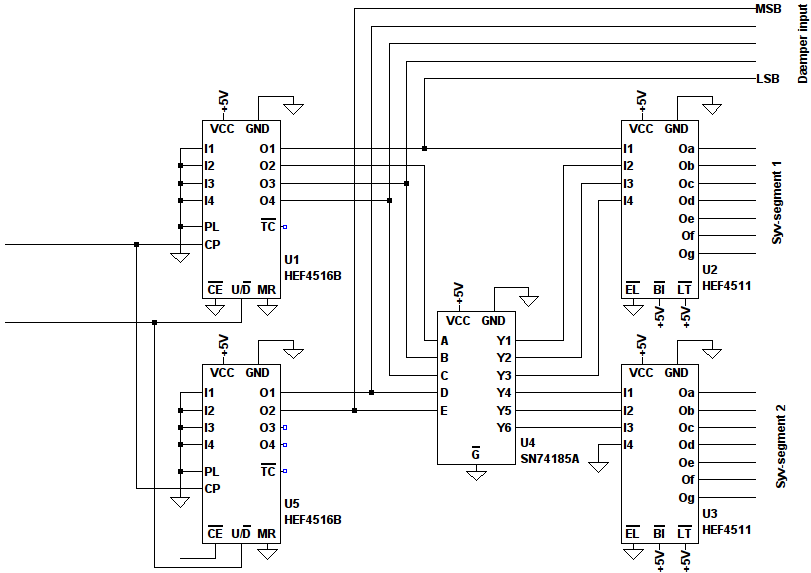
\includegraphics[width=\textwidth]{teknisk/volumenkontrol/taeller.png}
\caption{Diagram over tælleren og displaydriveren}
\label{fig:taeller}
\end{figure}

Tællerens opgave er at holde styr på hvad volumenniveauet er og diagrammet for den er vist på figur \ref{fig:taeller}. Der tælles op eller ned når der trykkes på én af de to volumenknapper. Hvor hurtigt der skal tælles, bestemmes af det AND'ede signal fra VCO'en og XOR-gaten. VCO'en fungerer som en clock på AND-gaten, mens XOR-signalet sørger for, at det kun er den ene knap der holdes nede. Hvis begge knapper holdes nede, vil XOR-signalet være lavt, og der vil intet signal blive sendt til tælleren. Om der skal tælles op eller ned, styres af et signal fra den knap der repræsenterer et ønske om en sænkning i volumeniveau. Hvis denne er nede, som den eneste knap, vil tælleren tælle ned af. Hvis denne ikke er nede, men XOR-signalet stadig er højt, betyder det at den anden knap er nede og tælleren vil derfor tælle op. Tælleren giver et binært output, som danner grundlag for hvad der vises i displayet og hvordan reguleringen af volumen indstilles. Tælleren der benyttes er en 4-bit tæller af typen HEF4516B \cite{hef4516b-datablad}. Da der skal bruges seks bit bruges to tællere.

Yderligere skal der også bruges kontrollogik, for at sikre tælleren ikke tæller for højt eller lavt og for at styre den anden tæller. Til at lave et endestop i den laveste ende af tællerens område, lægges alle tællerens output bits sammen i en OR-gate. Dette resultere i et nul, hvis tælleren står på nul. Der skal dog være mulighed for at tælle opad, når tælleren står på nul. Derfor skal UP/$\overline{\mathrm{DN}}$ signalet også med i OR-gaten, udgangssignalet vil nu være lavt når tælleren ikke må tælle nedad. Til at lave endestop i den høje ende, tages der udgangspunkt i en tæller værdi på 50, $110010_\mathrm{b}$. Da dette vil være maks værdien for tælleren er det kun de udgange der er høje, der er af betydning. Når disse og UP/$\overline{\mathrm{DN}}$ signalet bliver samlet i en NAND-gate vil resultatet kun være lavt når der ikke må tælles højere. Dette signal AND'es sammen med signalet for det lave endestop og CLK signalet, dette bevirker at der ikke kommer CLK signal til de to tællere hvis de har ramt et af endestoppene. I tabel \ref{tab:taeller} er sandhedstabellen for kontrollogikken til endestop opstillet.

\begin{table}[h]
\centering
\begin{tabular}{|l|l|l|l|l|l|l|l||r|}
\hline
UP/$\overline{\mathrm{DN}}$ & F & E & D & C & B & A & CLK & CP \\ \hline
0 & 0 & 0 & 0 & 0 & 0 & 0 & RaisingEdge & 0 \\
1 & 0 & 0 & 0 & 0 & 0 & 0 & RaisingEdge & RaisingEdge \\
0 & 1 & 1 & 0 & 0 & 1 & 0 & RaisingEdge & RaisingEdge \\
1 & 1 & 1 & 0 & 0 & 1 & 0 & RaisingEdge & 0 \\
\hline
\end{tabular}
\caption{Sandhedstabel for kontrollogik til endestop. A - D er output fra U1 og E - F er output fra U5}
\label{tab:taeller}
\end{table}

Tæller to, U5, skal kunne tælle når tæller ét, U1, har værdien 15, $1111_\mathrm{b}$, og UP/$\overline{\mathrm{DN}}$ er høj. Ved den næste puls på CP vil tæller ét gå til nul og tæller to vil tælle én op. Når tæller ét er nul og UP/$\overline{\mathrm{DN}}$ er lav, skal tæller to også kunne tælle. Ved næste puls på CP vil tæller ét gå til 15 og tæller to vil tælle én ned. I tabel \ref{tab:taeller2} er sandhedstabellen for kontrollogikken til tæller U5 opstillet.

\begin{table}[h]
\centering
\begin{tabular}{|l|l|l|l|l||r|}
\hline
UP/$\overline{\mathrm{DN}}$ & D & C & B & A & $\overline{\mathrm{CE}}$ \\ \hline
0 & 0 & 0 & 0 & 0 & 0 \\
1 & 0 & 0 & 0 & 0 & 1 \\
0 & 1 & 1 & 1 & 1 & 1 \\
1 & 1 & 1 & 1 & 1 & 0 \\
\hline
\end{tabular}
\caption{Sandhedstabel for kontrollogik til den anden tæller, U5. A - D er output fra U1}
\label{tab:taeller2}
\end{table}

Displaydriveren konverterer signalet fra tælleren til et signal der kan vises på de to 7-segment displays. Der konverteres fra tællerens binære output til BCD, Binary-coded decimal, for så at konvertere det til et signal de to 7-segment displays kan vise. Der benyttes en SN74185A \cite{sn74185a-datablad} til konverteringen fra binær til BCD. Fordelen ved at konvertere til BCD først er at denne konvertering også deler det binære tal op i to, en'ere og ti'ere. Disse to binære tal sendes igennem en 7-segmentsdriver, HEF4511 \cite{hef4511-datablad}, for at få et output der fungerer med 7-segmenterne. Displaydriveren er også vist på figur \ref{fig:taeller}.

\subsection*{Display}
\label{volumenkontrol-design-display}
Indstillingen af volumenkontrollen vises på to 7-segmenter. Dette er valgt, fordi disse er enkle at styre med simple kredsløb og det derfor ikke er nødvendigt med en microcontroller for at styre dem, som tilfældet havde været, hvis et LCD-display i stedet var blevet benyttet.

\subsection*{Dæmper}
\label{volumenkontrol-design-daemper}
Dæmperen er en en analog attenuator, som er sammensat af to sæt modstandsattenuatore, hver efterfulgt af en buffer. Dæmpningen indstilles ved at ændre, hvor signalet tages ud af de to modstandsattenuatore, ved brug af en analog multiplekser. Den første attenuator består af syv modstande, hvor der er en dæmpning på 8 dB mellem hver modstand. Den anden attenuatorer består af otte modstande, hvor der er en dæmpning på 1 dB mellem hver modstand. Det er således muligt at kombinere de to attenuatorer til at dæmpe signalet mellem 0 og 55 dB, med et interval på 1 dB. Diagrammet er afbilledet på figur \ref{fig:volumenkontrol_daemper} og modstandene derpå er beregnet i Appendiks C??.

\begin{figure}[h]
\centering
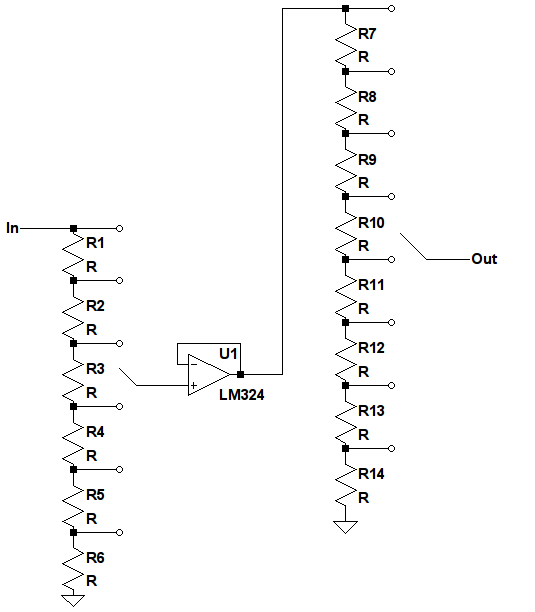
\includegraphics[width=\textwidth]{teknisk/volumenkontrol/daemper.png}
\caption{Diagram over dæmperen}
\label{fig:volumenkontrol_daemper}
\end{figure}

\clearpage
\subsection{Simulering}
\label{volumenkontrol-simulering}

På figur \ref{fig:volumenkontrol-diagram} er vist diagrammet, med komponent værdier, over volumenkontrollen til og med signalet til tælleren.

\begin{figure}[h]
\centering
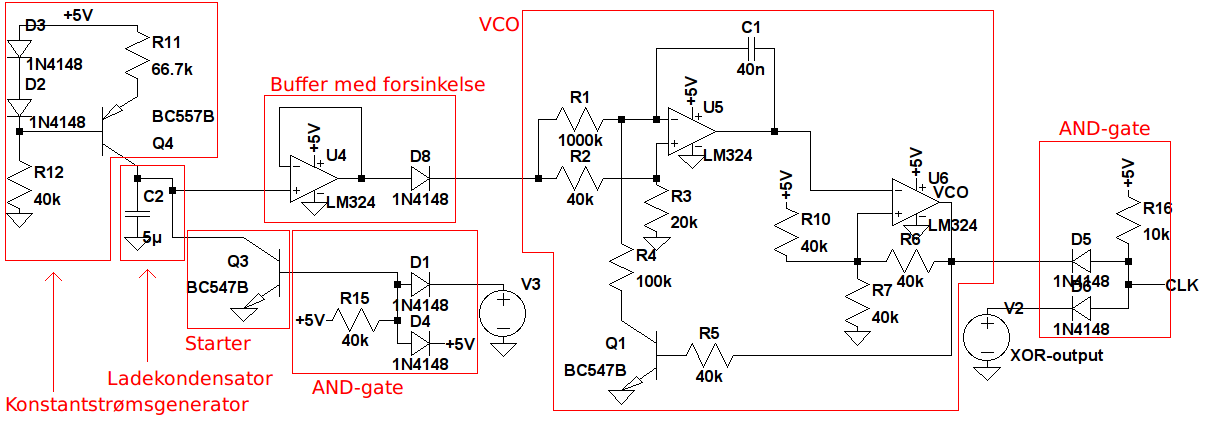
\includegraphics[width=\textwidth]{teknisk/volumenkontrol/diagram.png}
\caption{Diagram over volumenkontrollen}
\label{fig:volumenkontrol-diagram}
\end{figure}

På figur \ref{fig:vco-signal} ses resultatet af at påtrykke en konstant spænding på VCO'en. Dette resulterer i udgangen på integratoren, den blå kurve, svinger mellem schmitt-triggerens to niveauer med en fastdefineret frekvens. Det kan ses at plusindgangen på schmitt-triggeren, den røde kurve, er høj når integratorens udgang er opadgående og lav når den er nedadgående. 

\begin{figure}[h]
\centering
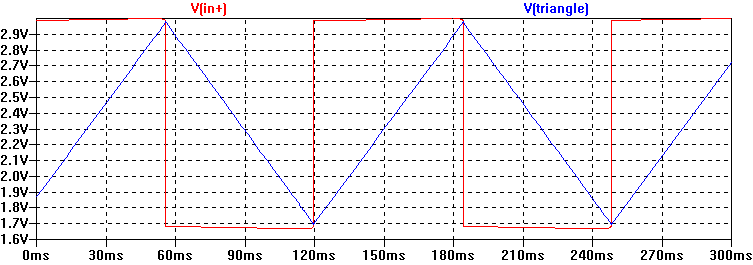
\includegraphics[width=\textwidth]{teknisk/volumenkontrol/vco-signal.png}
\caption{Integratorens udgang og plusindgangen på schmitt-triggeren}
\label{fig:vco-signal}
\end{figure}

Figur \ref{fig:stresstest} viser hvordan volumenkontrollen fungerer, når man trykker på en knap. Den blå graf, V(knap), viser knappens tilstand; når den er lav, er knappen trykket ned. Den lyseblå, V(clk) viser outputtet til clocken. Clocken på tælleren er flankestyret, hvilket vil sige, at der kun vil blive flyttet et trin, hver gang den lyseblå, V(clk) går fra lav til høj. Når knappen holdes nede, kan man se at kontrolspændingen, V(vc), stiger. Dette vil få spændingen på udgangen af integratoren, V(triangle), til at stige, indtil den rammer den høje trigger-spænding. Herefter vil spændingen falde igen, og oscillere hurtigere og hurtigere, i takt med at kontrolspændingen stiger. Ca. 3 sekunder efter at knappen trykkes ned, rammer kontrolspændingen sit max, som udregnet. Her vil udgangen på integratoren, og derfor også schmitt-triggeren, svinge med en frekvens på ca. 10 Hz.

\begin{figure}[h]
\centering
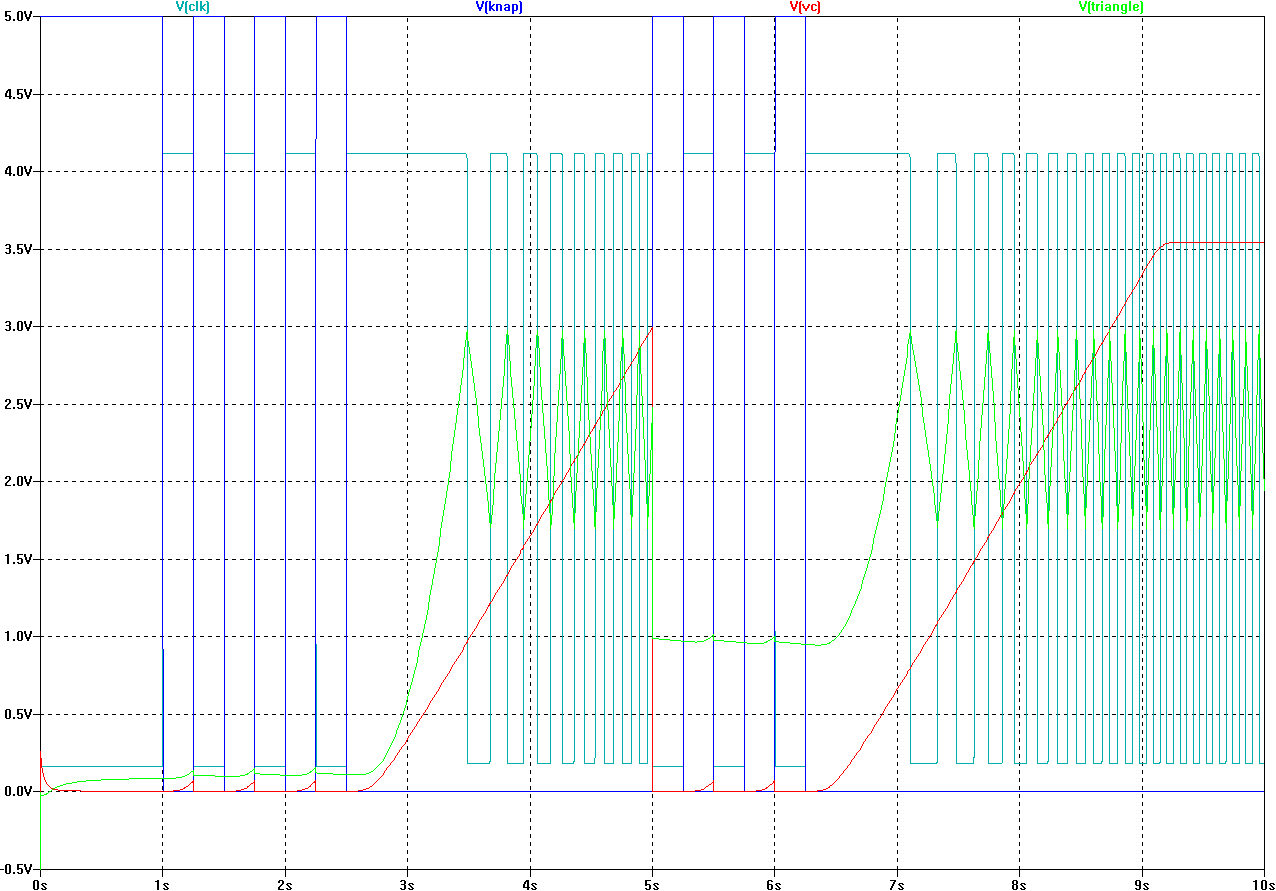
\includegraphics[width=\textwidth]{teknisk/volumenkontrol/stress-test.png}
\caption{Simulering af at trykke på og holde en knap nede.}
\label{fig:stresstest}
\end{figure}

På figur \ref{fig:konstantstroem} ses en simulering af konstantstrøms generatoren. Det er tydeligt at se, at konstantstrømsgeneratoren genererer en konstant strøm, Ic(Q4), indtil den ikke har et sted at løbe hen. Dette sker når kondensatoren er ladet op. Det er desuden tydeligt at se at kondensatoren, V(c2), bliver opladet lineært, med det samme knappen, V(knap), bliver trykket ned. 

\begin{figure}[h]
\centering
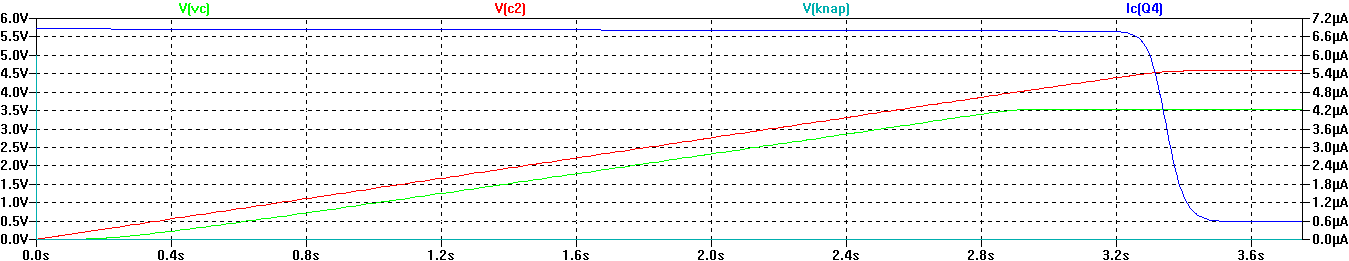
\includegraphics[width=\textwidth]{teknisk/volumenkontrol/konstantstroem.png}
\caption{Simulering af konstanstrømsgeneratoren}
\label{fig:konstantstroem}
\end{figure}